\subsection{Corpus}
\begin{frame}
  \frametitle{Columbia Games Corpus}
  \framesubtitle{Descripción}
  \begin{columns}
    \column{0.35\textwidth}
      \begin{figure}
        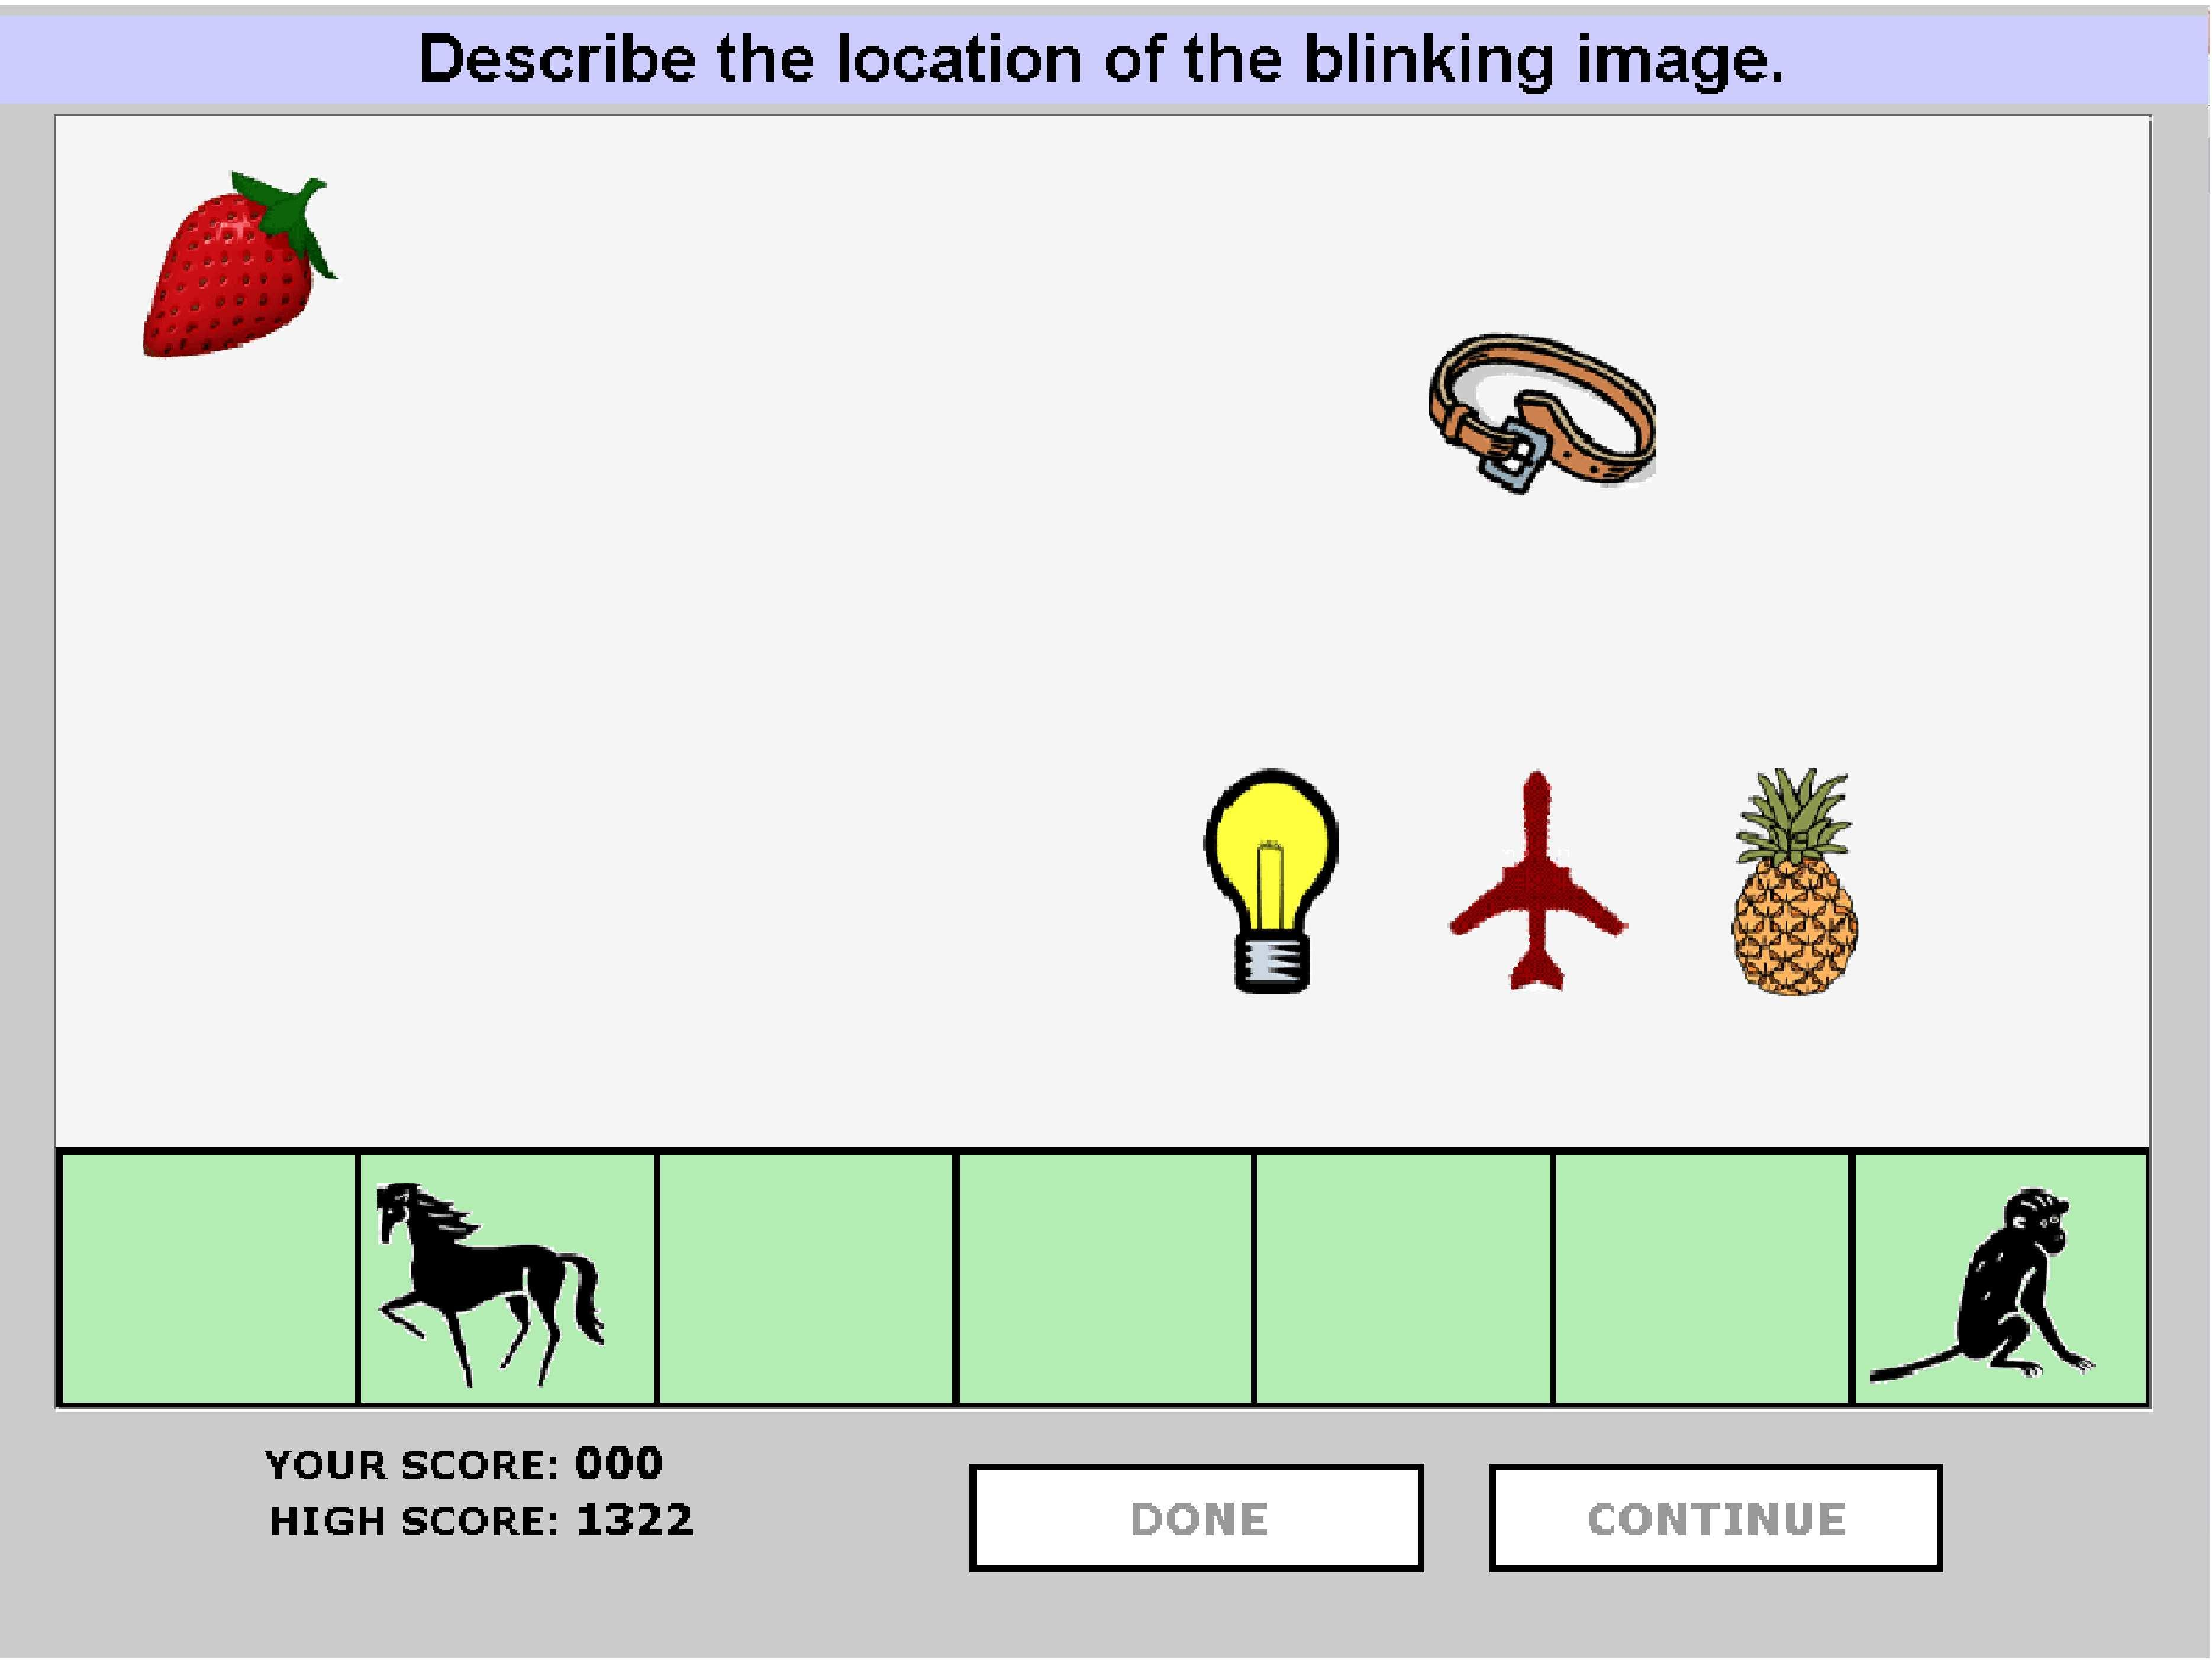
\includegraphics[width=\textwidth]{images/columbia_games_color.jpg}
      \end{figure}

    \column{0.65\textwidth}

    \begin{itemize}
      \item Corpus de conversaciones diádicas en Inglés Norteamericano
      \item 12 sesiones con 14 tareas/juegos cada una.
      \item En cada sesión, se sentó a dos participantes en una cabina profesional de grabación, y una cortina opaca colgando entre ellos para evitar la comunicación visual.
      \item Los participantes contaron con computadoras a través de las cuales interactuaban mediante juegos.
    \end{itemize}
  \end{columns}

\end{frame}


\begin{frame}
  \frametitle{Columbia Games Corpus}
  \framesubtitle{Juegos de objeto}
  \begin{columns}
    \column{0.35\textwidth}
      \begin{figure}
        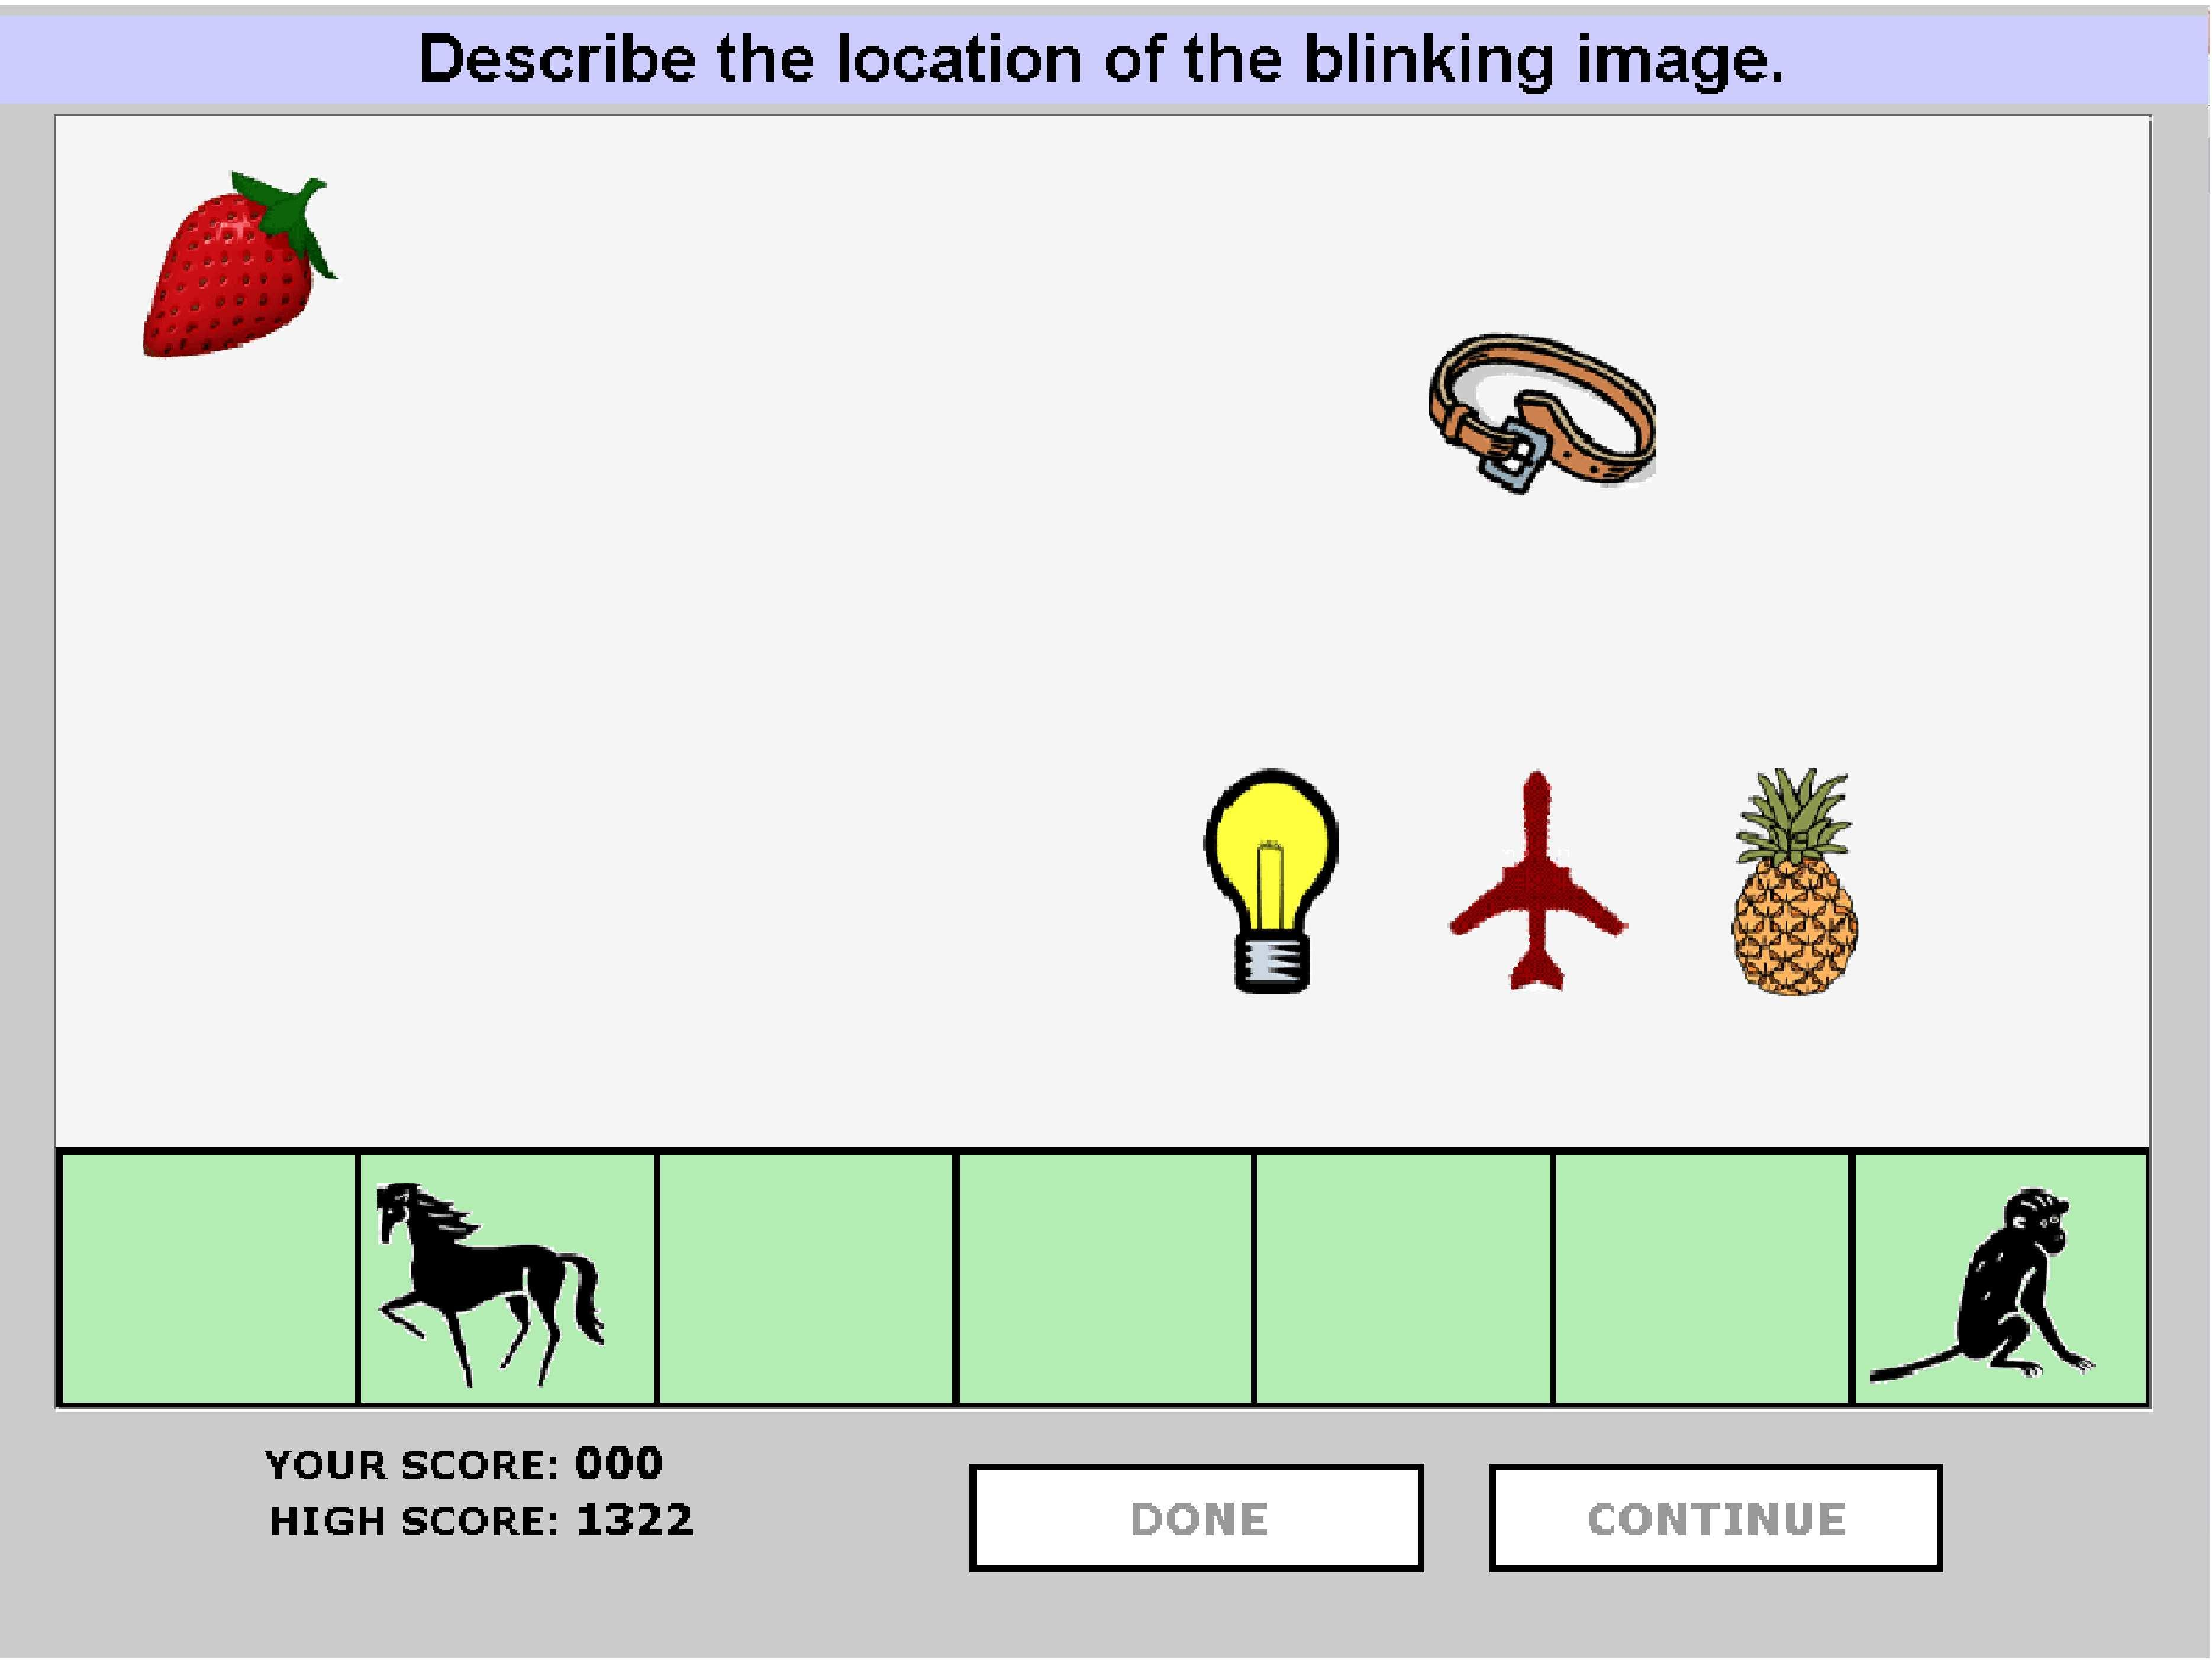
\includegraphics[width=\textwidth]{images/columbia_games_color.jpg}
      \end{figure}

    \column{0.65\textwidth}

    \begin{itemize}
      \item Dos roles: Descriptor y Seguidor
      \item En la pantalla, se ven entre 5 y 7 objetos en posiciones aleatorias
      \item El Descriptor ve uno más, titilante, del cual debe describir su posición
      \item El Seguidor debe mover la representación del objeto a la misma posición de la pantalla
      \item Finalmente, se puntúa de 1 a 100 el posicionamiento del objeto
    \end{itemize}
  \end{columns}
\end{frame}





\begin{frame}
  \frametitle{Columbia Games Corpus}
  \framesubtitle{Anotaciones sociales}

  Cinco anotadores escucharon el audio correspondiente a una tarea del juego y respondieron a varias preguntas sobre los sujetos:


\begin{table}
\adjustbox{max width=0.8\textwidth}{
\begin{tabular}{|l|l|}
  \hline

  \textbf{Nombre} & \textbf{Pregunta} \\
  \hline

  \svcontributes &  ¿el sujeto contribuye para el éxito del equipo?  \\ \hline
  \svengaged &  ¿el sujeto parece comprometido con el juego? \\ \hline
  \svclear &  ¿el sujeto se expresa correctamente? \\ \hline
  \svplanning &  ¿el sujeto piensa lo que va a decir? \\ \hline
  \svencourages &  ¿el sujeto alienta a su compañero? \\ \hline
  \svdifficult &  ¿el sujeto le hace difícil hablar a su compañero? \\ \hline
  \svbored &  ¿el sujeto está aburrido con el juego? \\ \hline
  \svdislikes &  ¿al sujeto no le agrada su compañero? \\ \hline
\end{tabular}
}
\end{table}

De cada una de estas preguntas obtenemos un puntaje de 0 a 5, para cada hablante de cada tarea.
\end{frame}


\begin{frame}
\frametitle{Extracción de features acústico-prosódicas}

Usando el software Praat \footnote{http://www.fon.hum.uva.nl/praat/} se extrajeron las variables acústico-prosódicas para cada segmento de habla

\begin{table}
\adjustbox{max width=0.8\textwidth}{
\centering
\begin{tabular} {|c|c|}
  \hline
  Variable & Descripción \\
  \hline
  \FOMEAN & Valor medio de la frecuencia fundamental \\\hline
  \FOMAX  & Valor máximo de la frecuencia fundamental \\\hline
  \ENGMEAN & Valor medio de la intensidad \\\hline
  \ENGMAX & Valor máximo de la intensidad \\\hline
  \NOISETOHARMONICS & Noise-to-harmonics ratio \\\hline
  \LOCALSHIMMER & Shimmer medido \\\hline
  \LOCALJITTER  & Jitter medido \\\hline
  \SYLAVG & Cantidad de sílabas por segundo \\\hline
  \PHONAVG & Cantidad de fonemas por segundo \\\hline
\end{tabular}
}
\end{table}
\end{frame}



\subsection{Modificaciones a TAMA}

\begin{frame}
\frametitle{TAMA}
\framesubtitle{Nuestras modificaciones}

\begin{itemize}
  \item Usamos un step de 8s y un tamaño de ventana de 16s, manteniendo el solapamiento del 50\%.
  \item A diferencia del trabajo original de Kousidis, utilizamos series con datos faltantes.
  \item Pero sólo nos quedamos con aquellas que tengan 5 o más puntos definidos.
\end{itemize}
\end{frame}


\begin{frame}
\frametitle{TAMA}
\framesubtitle{Cálculo de series de tiempo}

\begin{figure}
\centering
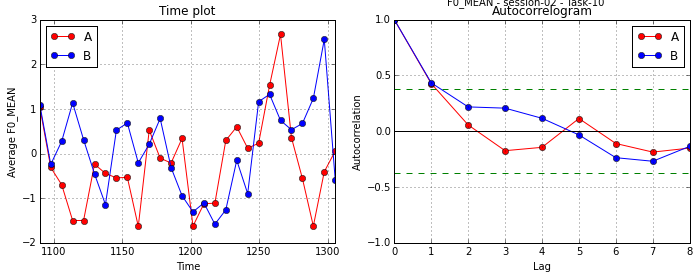
\includegraphics[height=3cm]{images/time_plot_with_autocorrelation.png}
\end{figure}



Para cada una de las variables acústico/prosódicas

\begin{itemize}
  \item Calculamos la serie de tiempo para ambos interlocutores por cada tarea
  \item Calculamos autocorrelogramas, y verificamos su estacionariedad
\end{itemize}
\end{frame}

\begin{frame}
\frametitle{TAMA}
\framesubtitle{¿Y el entrainment?}

  \begin{columns}
    \column{0.33\textwidth}
    \begin{figure}[t]
      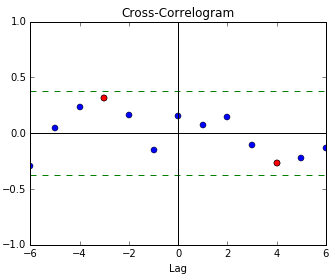
\includegraphics[scale=0.33]{images/cross_correlogram_2.png}
    \end{figure}
    \column{0.66\textwidth}

    Definimos dos medidas de entrainment

    \begin{align*}
      \fwentrainment{AB}^{(1)} &= r_s \text{ con s maximizando } |r_k|,  k > 0  \\
      \fwentrainment{BA}^{(2)} &= |\fwentrainment{BA}^{(1)}|
    \end{align*}

    Segunda métrica motivada por estudios sobre el disentrainment. Healey et al (2014) sugiere que puede ser una conducta de adaptación cooperativa.

    Levitan et al (2015) da más indicios en esa dirección.
  \end{columns}
\end{frame}

\begin{frame}
\frametitle{Entrainment y relación con variables sociales}

  Para analizar la relación entre las variables sociales ($V$) y el \emph{entrainment} ($\mathcal{E}$), planteamos un modelo de regresión lineal.

    \begin{equation}
      V_i \sim \beta_1 + \beta_2 \mathcal{E}_i
    \end{equation}

  Nuestra hipótesis es

  \begin{enumerate}
    \item Si $SV$ es una variable de carácter positivo, entonces $\beta_2 > 0$
    \item Si $SV$ es una variable de carácter negativo, entonces $\beta_2 < 0$
  \end{enumerate}
\end{frame}
